\newcommand{\lrv}{\vec{v}^{\,(p)}}

Two datasets were used for training and testing:

\begin{description}
    \item[The Qin dataset] is a dataset of 202 surfactants curated in a
          previous work, by \citet{qinPredictingCriticalMicelle2021}, by
          accumulating results from several publications. To the authors'
          knowledge, it is currently the largest public dataset of CMCs for
          several classes of surfactant collected at standard conditions in an
          aqueous environment between \SIrange{20}{25}{\celsius}. In this work,
          the data was further subdivided into two tasks: Qin-All, the entirety of
          the dataset, and Qin-Nonionics, which contains only the nonionic
          surfactants.

          The Qin data were split into training and test subsets; the training
          data were used to fit the models, whilst test data were `locked away'
          until it had been decided that the model was optimised, and the
          performance metrics on the test data were then used for evaluation. For
          some models, the training data were further split into optimisation and
          validation subsets; the optimisation data were used when calculating the
          loss function during model fitting. The validation data were used for
          on-the-fly evaluation of model performance during training, to determine
          how many iterations of the optimisation routine to use.

          To provide a consistent benchmark of model performance with
          the previous work \cite{qinPredictingCriticalMicelle2021}, the same
          train/test data splits were used as
          \citet{qinPredictingCriticalMicelle2021}. This will be referred to as
          the benchmarking test.

          After training these models, a sensitivity analysis was carried out.
          The data for each task were split using a repeated, stratified
          $k$-fold cross-validation. Each molecule was assigned a class based
          upon its molecular fingerprint, which will be described below, in the
          section on Extended connectivity fingerprints. The data were then
          split into $k$ folds of roughly equal size, and containing
          approximately the same percentage of molecules of each class, for $k
          \in (2, 5)$. For each fold, a model was trained using $k-1$ folds and
          evaluated on the remaining fold. This was repeated thrice for $k = 2$
          and twice for $k = 3$, each time with different randomisation, so that
          there were a similar number of models trained for each value of $k$.

    \item[The National Institute of Science and Technology (NIST) dataset]
          contains 43 unique surfactant systems and their aqueous CMCs, extracted
          from the work of \citet{mukerjeeCriticalMicelleConcentrations1971}. The
          original document compiles CMC measurements for each system across
          several temperatures and with various additives. Each measurement was
          given a quality rating depending on the authors' assessment of the
          experimental method; measurements with a sufficiently good rating were
          categorised as `suggested' measurements. The dataset used for this work
          was developed by taking the mean of the suggested CMC measurements
          between \SIrange{20}{25}{\degreeCelsius}, with no additives, for
          each surfactant system with measurements that fit these criteria. The
          surfactant systems that contained elements that were not present in the
          dataset (\ce{Mn}, \ce{Cs} and \ce{Mg}) were then pruned. The dataset is
          provided in the Supplementary Information.

          The NIST data were used exclusively for external validation. Several
          of the surfactant systems are not expected to be within the
          applicability domain of the models. This includes surfactants with
          counterions and combinations of functional groups that are not present
          in the training data. These data are included to test the robustness
          of the uncertainty quantification approach.
\end{description}

The number of each type of surfactant in the train and test subsets of the data are shown in Table~\ref{tab:data-split}. Only the models trained on the Qin-All dataset were evaluated on the NIST dataset, as it contained ionic compounds.

\begin{table}
    \centering
    \caption{The number of each type of surfactant contained in the train/test subsets of the CMC datasets. Missing entries mean no samples of that class.}
    \label{tab:data-split}
    \begin{tabular}{@{}llrrrr@{}} \toprule \multicolumn{2}{c}{Data subset} & \multicolumn{4}{c}{Number of}                                                    \\\cmidrule(r){1-2}\cmidrule(l){3-6}
               Task                                                    & Train/test                    & Nonionics & Anionics & Cationics & Zwitterionics \\\midrule
               Qin-All                                                 & Train                         & 110       & 30       & 31        & 9             \\
                                                                       & Test                          & 12        & 4        & 4         & 2             \\
               Qin-Nonionics                                           & Train                         & 110       &          &           &               \\
                                                                       & Test                          & 12        &          &           &               \\
               NIST                                                    & Train                         &           &          &           &               \\
                                                                       & Test                          & 12        & 23       & 6         & 2             \\\bottomrule
    \end{tabular}
\end{table}

As described in the Introduction, the QSPR pipeline needs molecular descriptors
and a functional form. The design processes for these are called \emph{feature
    engineering} and \emph{model selection}, respectively.

\subsection{Feature engineering}

In this work, two types of molecular descriptor are employed: extended
connectivity fingerprints (ECFPs)
\cite{rogersExtendedConnectivityFingerprints2010} and molecular graphs.

\subsubsection{Extended connectivity fingerprints (ECFPs)}

In the ECFP approach, the molecule is split into atomic environments up to a
given radius, $r$: each environment is centred on an atom and extends $r$ steps
along connecting bonds. The set of all environments in the training data up to
radius $r$ is extracted. The resulting feature vector, $\vec{c}$ for a molecule
is described by
\begin{equation}
    \label{eq:ecfp}
    c_m = \text{Count}(\mathcal{E}_m),
\end{equation}
where $\mathcal{E}_m$ represents the $m^\text{th}$ atomic environment.

A change in headgroup composition is, therefore, reflected in a change in
subgraph counts, and provided the new subgraph exists in our training data. The
model can adjust its prediction accordingly. Branch points in a carbon chain are
distinguished from main-chain groups, as they terminate in a \ce{CH} group
rather than \ce{CH2}.

ECFPs are similar to a segment-based approach; however, unlike segments or
groups, subgraphs can overlap. Whilst a group contribution approach requires
that a canonical `priority' of the groups be defined prior to featurising
molecules, by using ECFPs, the manual identification of important groups and
their priorities are skipped; feature importance determination is instead
delegated to the model.

Much like a group contribution approach, these fingerprints do not necessarily
distinguish between all positional or chain isomers, particularly with smaller
values of $r$, nor are stereoisomers treated differently.

A potential disadvantage with this approach, compared to group contributions, is
that the number of unique atomic environments is potentially very large relative
to the size of the data available, which poses a risk of overfitting.
Furthermore, larger environments necessarily envelop smaller ones, which means
that there is some duplicate information in the representation: the presence of
a \ce{(CH2)3} environment implies the presence of three \ce{CH2} environments,
so that there is multicollinearity. This redundancy can impede model fitting and
interpretation. However, these issues can be ameliorated using a process of
\emph{feature selection}, which will be discussed below.

ECFPs are commonly employed for determining molecular similarity through the use
of the Tanimoto similarity metric
\cite{tanimotoElementaryMathematicalTheory1958,bajuszWhyTanimotoIndex2015,butinaUnsupervisedDataBase1999}.
The Tanimoto similarity is a function of two binary fingerprints, so the
count-based ECFPs are first converted by $b_i = \min (1, c_i)$. That is, if an
atomic environment is present in a molecule, it is assigned a one; otherwise, it
is assigned zero. The Tanimoto similarity between molecules A and B is then
\begin{equation}
    S_{AB} = \frac{\vec{b}_A \cdot \vec{b}_B}{\vec{b}_A \cdot \vec{b}_A + \vec{b}_B \cdot \vec{b}_B - \vec{b}_A \cdot \vec{b}_B}.
\end{equation}

In the original work by \citet{tanimotoElementaryMathematicalTheory1958}, a
`distance coefficient' is defined based on the logarithm of the similarity of
two points; however, this is not a true distance metric as it does not satisfy
the triangle inequality. Instead, the Jaccard distance, $d_{AB} = 1 - S_{AB}$,
was employed to perform clustering of the molecules of the Qin dataset. The
pairwise distances between each feature-selected molecular fingerprint in the
Qin dataset were computed and the OPTICS clustering algorithm was then used to
assign a class to each of them \cite{ankerstOPTICSOrderingPoints1999}. The
algorithm was parameterised with a minimum cluster size of 4 molecules. Outlying
molecules, which did not fit into any other class, were assigned an `outliers'
class for the sake of the stratified splitting procedure.

The clusters must be assigned before determining the train/test splits for each
fold during the sensitivity analysis, so in order to provide a canonical cluster
assignment, the fingerprints resulting from the benchmarking test on the Qin-All
task were employed.

\subsubsection{Molecular graphs}

% In the case of the Stauff-Klevens model, the representation effectively has two
% components: the category of the headgroup, and the length of the tail group. The
% model technically distinguishes between isomers by imposing strict constraints
% on the structure of the molecules to which it can be applied: position and
% functional isomers correspond to distinctive categories, so that the model must
% learn independent parameters for each of them, and the constraint on the tail
% group means that chain isomers or the presence of non-alkyl groups in the carbon
% chain are not permitted. Mathematically, this representation can be formalised using
% a technique called \emph{one-hot encoding} and by defining the set of headgroups for which
% we have data, $\{h_i \mid 0 \leq i \leq N\}$. The encoding is a vector given by

% \begin{equation}
%     \label{eq:one-hot}
%     \vec{s}_i = \begin{cases}
%         1 & \text{if headgroup is } h_i \\
%         0 & \text{otherwise.}
%     \end{cases}
% \end{equation}

% Different headgroups therefore correspond to orthogonal encodings. If we have a
% set of trained parameters $\{A_i, B_i\}$ corresponding to headgroup $h_i$,
% Equation~\ref{eq:klevens} can be rewritten as

% \begin{equation}
%     \log X_{cmc} = \mathbf{W}\vec{s} \cdot \begin{bmatrix}
%         1 \\ -n_c
%     \end{bmatrix},\quad \mathbf{W} = \begin{pmatrix}
%         A_1 & A_2 & \dots & A_N \\
%         B_1 & B_2 & \dots & B_N \\
%     \end{pmatrix}.
% \end{equation}

% We can try to make the approach more general by decomposing a molecule into
% smaller sets of \emph{atomic environments} and representing it by the number of
% each of these constituents. Because certain groups of atoms and bonds are common
% in organic surfactants, the resulting feature vectors are not orthogonal, and we
% can apply the model even when we have made small changes to the headgroup, or
% introduce branching and other functional groups to the tail.


A molecular graph is a structure that describes the entire topology of a
molecule and it is a popular choice for cheminformatics as well as visualisation
of molecular structure. Each atom is considered a \emph{node} and each bond an
\emph{edge}. Rather than having a single feature vector to describe the molecule
as a whole, each atom is assigned its own feature vector, $\vec{v}_i$, based on
properties such as its element, hybridisation state, charge, etc. The same set
of atomic features were used here as in the work by
\citet{qinPredictingCriticalMicelle2021}. It is for this reason that the
molecules in the NIST data containing elements that were not in the training
data were excluded; the atomic representation includes a fixed-length one-hot
encoding of the element number, and the new elements cannot be encoded without
modifying the model after training. These feature vectors are concatenated into
a node feature matrix, $\mathbf{V}$. The graph's structure is then defined by a
binary adjacency matrix, $\mathbf{A}$:

\begin{equation}
    \label{eq:adjacency-mat}
    \mathbf{A}_{ij} = \begin{cases}
        1 \quad \text{if } i \text { bonded to } j \text{, or } i = j \\
        0 \quad \text{otherwise.}
    \end{cases}
\end{equation}

Molecular graphs are natural representations to visualise; see Figure~\ref{fig:mol-graph}. This is exact description of the molecule's topology enables an atomistic machine learning approach.

\begin{figure}
    \centering
    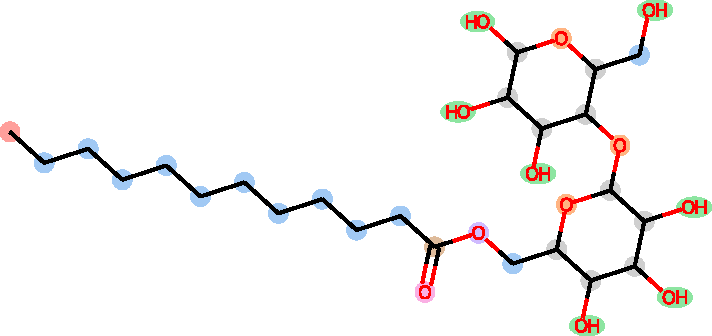
\includegraphics[width=.8\linewidth]{images/molecular-graph.pdf}
    \caption{A molecular graph of 6-\textit{O}-dodecanoyl-maltose. Atoms are
        highlighted based on their feature vectors, $\vec{v}_i$, so that equal
        feature vectors have the same colour.}
    \label{fig:mol-graph}
\end{figure}

\subsection{Model selection}

\subsubsection{ECFP model}

Based on the prior knowledge encoded in Equation~\ref{eq:klevens}, it is
assumed that certain atomic environments have a linear relationship to $\log X_{cmc}$. It therefore seems justified to apply a linear model to the ECFP fingerprints described in Equation~\ref{eq:ecfp}:
\begin{equation}
    \label{eq:linear-ecfp}
    \log X_{cmc} = \vec{w} \cdot \vec{c} + b,
\end{equation}
where $\vec{w}$ is a trained weights vector, the elements of which correspond to the contribution of an atomic environment to the CMC, and $b$ is an intercept (or \emph{bias} term).

However, the issues of the large feature vector size and multicollinearity must
be addressed. To that end, a process of \emph{feature selection} was applied,
whereby a subset of the atomic environments were selected for use in the model.
There are several approaches to feature
selection\cite{liFeatureSelectionData2017}; here, we chose an approach based on
\emph{regularisation}.

In this approach, we include a term in the loss function that depends on the
norm of $\vec{w}$. The two types of constraints considered are $\ell_1$ and
$\ell_2$ regularisation, which correspond to the inclusion of $\ell_1$ and
$\ell_2$ norms, respectively. Concretely, the ElasticNet
\cite{zouRegularizationVariableSelection2005} loss function was employed:

\begin{equation}
    \label{eq:elastic}
    \min_{\vec{w}} { \frac{1}{2n_{\text{samples}}} \left \Vert \mathbf{C}\vec{w} + \vec{b}- \vec{y} \right \Vert_2 ^ 2 + \alpha\rho \left \Vert \vec{w} \right \Vert_1} + \frac{\alpha(1 - \rho)}{2} \left \Vert \vec{w} \right \Vert_2^2,
\end{equation}

where $n_{\text{samples}}$ is the number of training samples; $\vec{y}$ are the
training data's true values of $\log X_{cmc}$; $\vec{b}$ is a vector with
elements all equal to $b$; and $\alpha$ and $\rho$ are user-defined
hyperparameters describing the degree of regularisation ($\alpha \geq 0$), and
the proportions of the regularisation terms ($0 < \rho < 1$), respectively.
$\mathbf{C}$ are the standardised training data feature vectors,
$\{\vec{c}^{\,\prime}_n \,|\, 1 \leq n \leq n_\text{samples}\}$, stacked
row-wise into a matrix.

Standardising the environment counts ensures that they have zero mean and unit variance:
\begin{equation}
    \label{eq:standard-scaling}
    {c}^{\,\prime}_m = \frac{c_m - u_m}{s_m},
\end{equation}
where $u_m$ and $s_m$ are the mean and standard deviation of the number of $\mathcal{E}_m$ in each molecule in the training data. This standardisation is necessary to ensure that the regularisation term is not dominated by
environments with high variance and that it accounts for common and uncommon environments alike.

By imposing the $\ell_1$ penalty, the model is biased towards learning a
\emph{sparse} weight vector: many of its elements will be negligible. The
corresponding features can be removed from the representation. Meanwhile, the
$\ell_2$ penalty means that a `grouping' effect is achieved, ensuring that
highly correlated groups all get given similar weights, rather than discarding
some of them, and it also ensures that there is no upper bound on the number of
groups that the model includes. Both of these are potential issues when using
only an $\ell_1$ norm in the loss function
\cite{efronLeastAngleRegression2004,zouRegularizationVariableSelection2005}.

To determine the best values for $\alpha$ and $\rho$, 5-fold cross-validation of
the training data was used. This was applied for a range of $\alpha$ and $\rho$
combinations, and the combination that achieved the lowest average
mean-squared-error was then used to train a model using the entirety of the
training data. The hyperparameter search space is defined in the Supplementary
Information.

The features with non-negligible fitted weights from ElasticNet were then selected for use in the final linear model. This model, ridge regression, uses just $\ell_2$ regularisation so that all of the weights are non-negligible, but we
still address the issue of multicollinearity \cite{mcdonaldRidgeRegression2009}:
\begin{equation}
    \min_{\vec{w}} \left \Vert \mathbf{C} \vec{w} + \vec{b} - \vec{y} \right \Vert_2^2 + \alpha \left \Vert \vec{w}\right \Vert_2^2.
\end{equation}
A similar cross-validation method to the one described above was used to determine the best $\alpha$ parameter, but using leave-one-out cross-validation, whereby $k=n_\text{samples}-1$. Because only one hyperparameter needs to be determined. There are far fewer trials per
fold, and therefore a greater number of folds can be used.

It was empirically observed that the combination of ElasticNet feature selection and a final regression with the simpler ridge regression model yielded better results, likely due to using a larger number of folds when determining the best value for $\alpha$. Both models were implemented using scikit-learn \cite{pedregosaScikitlearnMachineLearning2011}.

\subsubsection{Molecular graph model}

The basic topology of the graph neural network (GNN) used in this work was identical to the one used by \citet{qinPredictingCriticalMicelle2021}. That is, the first step of the model consists of a stack of graph network layers, which mutate the node features in a molecular graph based on those of bonded atoms.
These layers employ the graph convolution network (GCN) architecture introduced by \cite{kipfSemiSupervisedClassificationGraph2017a}. Layer $l$ computes a new node feature matrix, $\mathbf{V}^{(l)}$, based on the adjacency matrix, $\mathbf{A}$:
\begin{equation}
    \mathbf{V}^{(l)} = \mathbf{D}^{-1/2} \mathbf{A} \mathbf{D}^{-1/2} \mathbf{V}^{(l-1)} \mathbf{W}^{(l)} + \mathbf{b}^{(l)}.
\end{equation}
Here, $\mathbf{W}^{(l)}$ and $\mathbf{b}^{(l)}$ are the weights and biases,
respectively, of layer $l$ and we have also introduced the degree matrix,
\begin{equation}
    D_{ii} = \sum_j A_{ij},
\end{equation}
so that the term $\mathbf{D}^{-1/2} \mathbf{A}
    \mathbf{D}^{-1/2}$ effectively normalises the adjacency matrix based on
the degree of each atom.

$\mathbf{V}^{(1)}$, therefore, encodes not only information about the atom itself but its bonded neighbours. This information is used in the subsequent graph convolution so that $\mathbf{V}^{(2)}$ encodes information about the
2\textsuperscript{nd} order neighbourhood, \emph{et cetera}. The number of graphs layers, $L$, therefore dictates the `radius' around each atom that is considered in computing the final feature vector, analogous to creating an ECFP, except that the $i^\text{th}$ atomic environment is characterised by a continuous, \emph{latent} vector, $\vec{v}^{\,(L)}_i$.

The next step is a pooling layer, which converts the graph to a single \emph{latent representation vector}, $\lrv{}$, losing the explicit topological information. Several choices of pooling function were trialled:

\begin{description}
    \item[Mean pooling] was employed by \citet{qinPredictingCriticalMicelle2021}. It computes the average
          over all atoms' latent feature vectors.
    \item[Sum pooling] computes the sum of all atoms' latent feature vectors.
          This is the most analogous to the ECFPs in that the contribution of an atomic environment scales linearly with the number of times it occurs
          in the molecule.
    \item[Gated attention pooling] applies an \emph{attention} mechanism to decide which environments
          are relevant to the prediction \cite{liGatedGraphSequence2017}:
          \begin{equation}
              \lrv{} = \sum_i^N \sigma\left(\mathbf{W}_1 \vec{v}_i^{\,(L)} + \vec{b}_1 \right) \odot \left(\mathbf{W}_2 \vec{v}_i^{\,(L)} + \vec{b}_2 \right),
          \end{equation}
          where $\mathbf{W}_1$ and $\mathbf{W}_2$ are trained weights and
          $\vec{b}_1$ and $\vec{b}_2$ are biases, $\sigma$ is the sigmoid
          activation function, $N$ is the number of atoms in the molecule, and
          $\odot$ represents element-wise multiplication.
    \item[Attention sum pooling] is a simpler variation of the above. By using a
          softmax function, it performs a weighted average of the atomic environments'
          contributions:
          \begin{align}
              \mathbf{X} = \mathrm{softmax}(\mathbf{V}^{(L)}\vec{w}), \\
              \lrv{} = \sum_i^N \mathbf{X}_i \cdot \vec{v}^{\,(L)}_i,
          \end{align}
          where $\vec{w}$ are trained weights.
\end{description}

After training the model, $\lrv{}$ effectively acts as a machine-learned representation of the molecule that captures only the information about its topology and composition that is useful for predicting the CMC. Finding an optimised representation is a feature of neural networks that happens implicitly during training, called \emph{representation learning} \cite{goodfellowRepresentationLearning2016}.
The final step is a readout neural network: a multi-layer perceptron which acts as a nonlinear approximator to map this
latent representation vector to the CMC property prediction. Each layer in this neural network, called a `dense' layer, outputs a new vector, $\vec{v}^{(l)}$:
\begin{equation}
    \vec{v}^{(l)} = \mathbf{W}^{(l)}\vec{v}^{\,(l-1)} + \vec{b}^{\,(l)},
\end{equation}
The full network's architecture is illustrated in Figure~\ref{fig:model-topology}. The model was implemented using the open-source library Spektral\cite{grattarolaGraphNeuralNetworks2020} and optimised using an Adam optimiser \cite{kingmaAdamMethodStochastic2017a}.

\begin{figure}
    \centering
    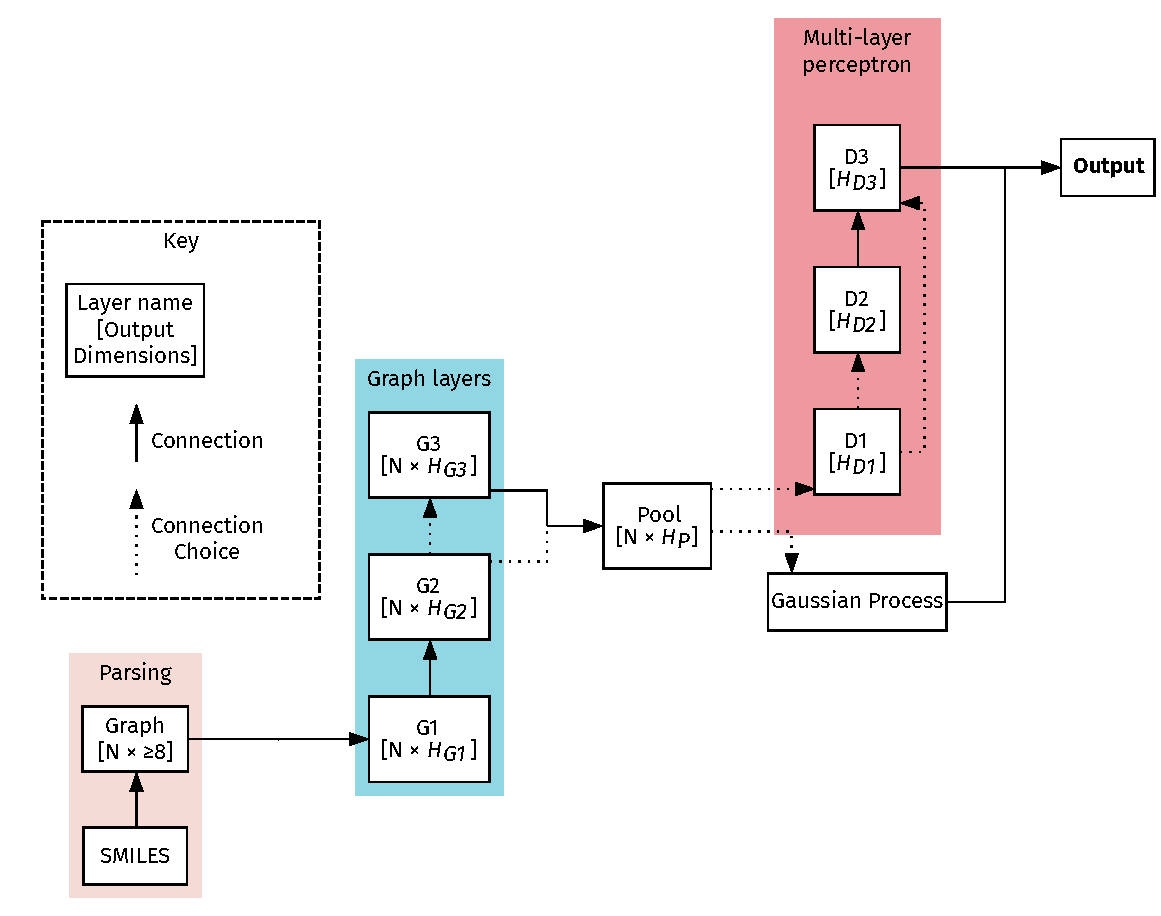
\includegraphics[width=\textwidth]{images/model_graph.pdf}
    \caption{Schematic of the neural network architecture. Here, $N$ represents
        the number of constituent atoms/ions in the input molecule and $H$
        represents a hyperparameter. The size of the pooling layer output, $H_P$, is
        only independent in the case of a gated attention-pooling layer. Otherwise,
        it is equal to the number of columns of the graph layer that feeds into it
        ($H_{G2}$ or $H_{G3}$).}
    \label{fig:model-topology}
\end{figure}

A neural network's topology describes the types of layers used, i.e. their functional form and the connection between them. Layers that are parameterised by a weight matrix, $\mathbf{W}$, may have different `sizes', meaning that the
dimensionality of their output is arbitrary and can be adjusted by changing the dimensions of $\mathbf{W}$. The graph layers, dense layers and the gated attention pool all have this property. These sizes, the type of pooling layer
and the number of each graph and dense layer, are all hyperparameters that can be adjusted prior to training. To determine the best combination of hyperparameters for predicting CMCs, an automated searching procedure was
employed.

\subsubsection{Optimising GNN hyperparameters}

The Hyperband approach \cite{liHyperbandNovelBanditBased2018}, implemented in Keras Tuner \cite{cholletKeras2015}, was used to select a good combination of hyperparameters for the model. Hyperband provides a way to efficiently evaluate
the performance of a large search space of hyperparameter configurations. The algorithm assesses several combinations of hyperparameters, initially allocating only a small number of resources to each trial. The hyperparameters for the
trials with the best performance are then allocated more resources, whilst the remainder is discarded. A reduction factor of 3 was chosen, meaning that $2/3$ of the trials were discarded after each iteration. This procedure iterates until the best configuration is found.

The algorithm can be executed multiple times if resources are available to obtain a more reliable result; the training procedure is stochastic, and therefore the performance of two trials with the same hyperparameters may be different. In this case, a single run was performed. The training data was partitioned into an optimisation subset and a validation subset in a ratio of 9:1. The trials were fit to the optimisation subset and evaluated based on the RMSE of their predictions on the validation subset.
The best hyperparameters determined on the benchmark tasks were then used during the sensitivity analysis.

\subsubsection{Adding uncertainty with a Gaussian process}

To improve the model's reliability, a \emph{surrogate} model was employed that could yield uncertainty estimates alongside CMC predictions. The approach is based on the Convolution-Fed Gaussian Process of \citet{tranMethodsComparingUncertainty2020}. The model first computes the latent representation vector, $\lrv{}$, of an input molecule using a trained GNN. $\lrv{}$ is then standardised, similar to Equation \ref{eq:standard-scaling},
but in this case the standardisation applies across each latent feature, $n$:
\begin{equation}
    v^{(p)\,\prime}_n = \frac{v^{(p)}_n - u_n}{s_n}.
\end{equation}
Again, $u_n$ and $s_n$ were determined from the training molecules' latent representations.

The standardised latent representation vectors of the training data serve as index points for a Gaussian process (GP); see Figure~\ref{fig:model-topology}.
The GP's predicted mean and standard deviation define a predicted normal distribution of a molecule's CMC, $\log X_{cmc} \sim \mathcal{N}(\mu, \sigma)$.

In this work, the GPs  were defined using a Mat\'ern kernel with parameter $1/2$, and a fixed noise variance of \num{1e-5}. Furthermore, the multi-layer perceptron component of the GNN used to calculate $\lrv{}$ was employed as the GP's mean function.
The kernel parameters were optimised with an Adam optimiser \cite{kingmaAdamMethodStochastic2017a}.
The same optimisation/validation splitting was used as for the GNN hyperparameter search and training was stopped after \num{1000} iterations without improvement in the validation predictions' RMSE, or after a total of \num{5000} iterations. This implementation was based on GPFlow \cite{matthewsGPflowGaussianProcess2017}.

\subsubsection{Visualising the latent space}

In order to better understand the model's interpretation of chemical space, we
implement a technique to exploit the GP's kernel, optimised during training, to
plot the molecules in 2D space in a way that respects the model's perception of
their `similarity'. This approach is inspired by
\citet{isayevMaterialsCartographyRepresenting2015}, who compared the
fingerprints of several inorganic compounds to develop so-called materials
catrograms. However, by employing the machine-learned latent representations of
molecules, the cartogram instead reflects molecular similarities learned by the
model itself.

Once having trained the GP, the learned kernel function was computed between
every pair of molecules in the combined data, NIST and Qin. These kernel values
were then normalised within the range $[0, 1]$. Each molecule was then assigned
a node in a graph and these were connected by edges. Each edge was given a
weight that was equal to the normalised kernel value between the two nodes it
connected.

This was the starting condition for computing a \emph{force-directed graph
    layout}. The nodes are initialised with a set of 2D coordinates that is
uniformly distributed and they are moved according to forces acting upon them;
primarily an attractive force that acts along the edges. In addition, there are
pairwise repulsive forces acting amongst the nodes that serves to ensure that
the equilibrium distance between two nodes is non-zero. In this work, the Force
Atlas 2 algorithm was employed
\cite{jacomyForceAtlas2ContinuousGraph2014,bastianGephiOpenSource2009}.